\documentclass[12pt]{article}
\usepackage{graphicx}
\usepackage{geometry}
\usepackage{setspace}
\usepackage{titlesec}
\usepackage{tocloft}
\usepackage{fancyhdr}
\usepackage{hyperref}
\usepackage{xcolor}
\usepackage[T1]{fontenc}
\usepackage[utf8]{inputenc}
\usepackage[ngerman]{babel}

\geometry{a4paper, margin=2.5cm}
\setstretch{1.5}
\titleformat{\section}[block]{\LARGE\bfseries\color{black}}{}{0em}{\filcenter}
\titlespacing*{\section}{0pt}{3.5ex plus 1ex minus .2ex}{2.3ex plus .2ex}
\renewcommand{\cftsecleader}{\cftdotfill{\cftdotsep}}
\renewcommand{\contentsname}{Inhaltsverzeichnis}
\renewcommand{\cftaftertoctitle}{\par\nobreak\bigskip\bigskip\bigskip}
\setlength{\cftbeforesecskip}{0.5em}
\setlength{\cftaftertoctitleskip}{2cm}
\hypersetup{
    colorlinks=true,
    linkcolor=blue,
    filecolor=magenta,
    urlcolor=cyan,
}

\pagestyle{fancy}
\fancyhf{}
\fancyhead[R]{\thepage}
\fancyhead[L]{\nouppercase{\leftmark}}
\renewcommand{\headrulewidth}{0pt}
\fancyfoot[C]{\thepage}
\renewcommand{\footrulewidth}{0pt}

\definecolor{lightgray}{RGB}{240,240,240}

\begin{document}

\begin{titlepage}
    \centering
    \vspace*{3cm}
    {\Huge\bfseries\textcolor{blue}{\MakeUppercase{ Die Magische Universität: Ein Jahr im Verborgenen }}\par}
    \vspace{0.5cm}
    {\Large\textit{ Maja Schmidt }\par}
    \vfill
    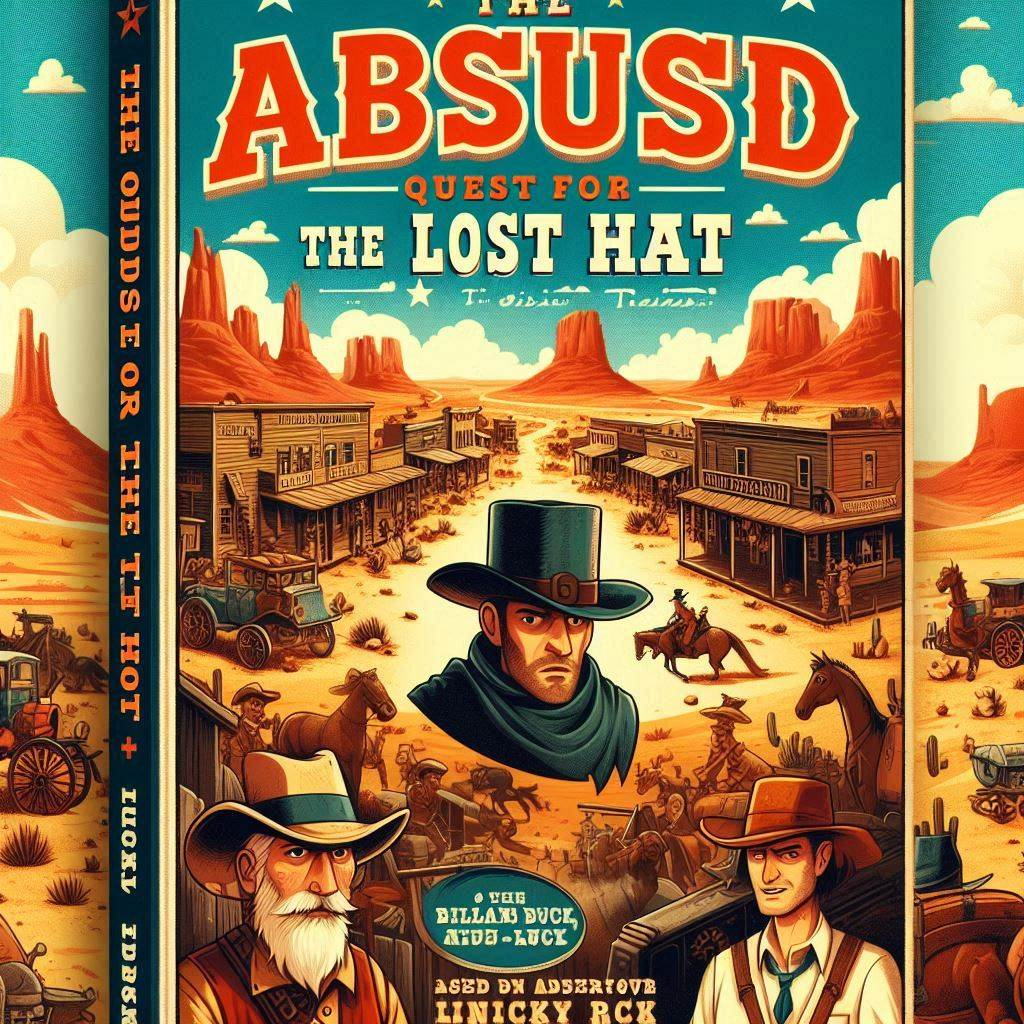
\includegraphics[width=0.9\textwidth]{ cover.jpg }
    \vfill
    \today
\end{titlepage}

\section*{Autorenvita}
\vspace{4cm}
Maja Schmidt ist eine bekannte und erfahrene Autorin von Fantasy-Büchern, die sich auf das Thema Studentenleben spezialisiert hat. Mit einer Leidenschaft für magische Welten und tiefgründige Charaktere hat sie bereits zahlreiche Leser*innen in ihren Bann gezogen. Ihre Geschichten zeichnen sich durch eine perfekte Mischung aus Abenteuer, Magie und den alltäglichen Herausforderungen des Studentenlebens aus.

\clearpage
\tableofcontents
\clearpage


\section{ Die Entdeckung der Magischen Fakultät }
Lukas Weber kämpfte sich durch die überfüllten Gänge der Universität von Eldoria. Der Alltag eines Studenten war nicht leicht, besonders wenn man zwischen Vorlesungen, Hausarbeiten und einem Nebenjob jonglieren musste. Eines Abends, als er auf dem Weg zurück zu seinem Wohnheim war, bemerkte er eine unscheinbare Tür, die er zuvor nie gesehen hatte. Neugierig öffnete er sie und fand sich in einem Raum voller alter Bücher und seltsamer Artefakte wieder. 'Was ist das hier?', murmelte er. Plötzlich hörte er eine Stimme hinter sich. 'Willkommen, Lukas', sagte Professor Alaric Stern. 'Du hast die magische Fakultät entdeckt.' Lukas starrte Professor Stern an, unfähig, ein Wort herauszubringen. 'Magische Fakultät?', fragte er schließlich. 'Ja, Lukas', antwortete Professor Stern mit einem geheimnisvollen Lächeln. 'Du hast eine Welt entdeckt, die nur wenigen zugänglich ist.' Plötzlich trat eine junge Frau mit langen, dunklen Haaren aus dem Schatten. 'Ich bin Mara Fischer', stellte sie sich vor. 'Willkommen in unserer Welt.' Lukas fühlte sich überwältigt, aber auch fasziniert. 'Was bedeutet das alles?', fragte er. 'Es bedeutet', sagte Professor Stern, 'dass du eine besondere Gabe hast, Lukas. Und wir werden dir helfen, sie zu entfalten.' Lukas begann seine ersten magischen Lektionen unter der strengen Aufsicht von Professor Stern. 'Konzentriere dich, Lukas', ermahnte der Professor, als Lukas versuchte, einen einfachen Zauber zu wirken. Mara stand neben ihm und flüsterte: 'Du schaffst das, nur nicht aufgeben.' Plötzlich betrat Felix Müller den Raum und warf Lukas einen abschätzigen Blick zu. 'Na, der Neue hat wohl Schwierigkeiten?', spottete er. Lukas ignorierte ihn und konzentrierte sich erneut. Mit einem tiefen Atemzug gelang ihm der Zauber, und ein kleines Licht erschien in seiner Hand. 'Gut gemacht', lobte Professor Stern. Lukas lächelte stolz.

\section{ Prüfungen und Geheimnisse }
Lukas stand nervös vor der ersten Prüfung. Professor Stern erklärte: 'Diese Prüfung wird eure magischen Fähigkeiten auf die Probe stellen.' Mara flüsterte: 'Du schaffst das, Lukas.' Felix grinste spöttisch: 'Mal sehen, ob der Neue das hinkriegt.' Lukas atmete tief durch und begann den Zauber. Plötzlich flackerte das Licht und er verlor die Kontrolle. 'Konzentriere dich!', rief Professor Stern. Mit einem letzten Kraftakt stabilisierte Lukas den Zauber. 'Gut gemacht', sagte der Professor. Felix schaute beeindruckt, aber sagte nichts. Lukas fühlte sich gestärkt. Nach der Prüfung saßen Lukas, Mara und Felix in der Mensa. 'Das war knapp', sagte Lukas und rieb sich die Schläfen. Mara nickte zustimmend: 'Du hast dich gut geschlagen.' Felix, der bisher still gewesen war, schaute auf und sagte: 'Vielleicht bist du doch nicht so schlecht, Weber.' Lukas lächelte überrascht. 'Danke, Felix.' Plötzlich betrat Professor Stern den Raum. 'Ich muss mit euch sprechen. Es gibt etwas, das ihr wissen müsst.' Die drei sahen sich an, ihre Neugier geweckt. Professor Stern führte die drei in einen abgelegenen Raum der Fakultät. 'Es gibt eine Bedrohung, die unsere Welt gefährdet', begann er. 'Ein uraltes Artefakt wurde gestohlen.' Mara runzelte die Stirn. 'Wer könnte so etwas tun?' Stern seufzte. 'Ein ehemaliger Schüler, der die dunklen Künste studiert hat.' Lukas spürte eine Mischung aus Angst und Entschlossenheit. 'Was können wir tun?' Felix, der bisher skeptisch war, nickte. 'Wir müssen zusammenarbeiten.' Stern lächelte schwach. 'Genau das. Ihr seid unsere einzige Hoffnung.'

\clearpage

\section*{Metadaten}
\colorbox{lightgray}{
    \begin{minipage}{\dimexpr\textwidth-2\fboxsep}
        \vspace{1cm}
        \begin{itemize}
            \item Name des Buches: Die Magische Universität: Ein Jahr im Verborgenen
            \item Name des Autors: Maja Schmidt
            \item Name des Herausgebers: Mark Zimmermann
            \item Name des Verlags: HdM AI Technologies
            \item Adresse des Verlags: Nobelstraße 10, 70569 Stuttgart
            \item Datum der Veröffentlichung: 2023-10-10
        \end{itemize}
        \vspace{1cm}
    \end{minipage}
}

\end{document}